%\documentclass[titlepage,a4paper,12pt]{book}
%\usepackage[utf8]{inputenc}
%\usepackage[catalan]{babel}
%\usepackage{graphicx}
%\usepackage{verbatim}
%\usepackage{marvosym}
%\usepackage{amssymb, amsmath} 
%\usepackage{listings}
%\usepackage{textcomp}
%\usepackage[]{color}


%\begin{document}
%\tableofcontents  %%Index

\chapter{GEP} % (fold)
\label{cha:GEP}

\section{Objectius} % (fold) Objectius?
\label{sec:Introduccio}
Tot seguit es presentarà un projecte en el que s'ha utilitzat una tècnica
molt pionera derivada de la programació genètica anomenada ``Genetic
Expression Programming'' (GEP).  A falta d'un nom millor hem tractat el
problema amb el nom de \texttt{GEP}.

En aquest projecte apliquem Genetic Expression Programming per a descobrir
fórmules analítiques a partir de resultats empírics o bé mostrejos que tenim
a priori de característiques que tenen les molècules en funció de paràmetres
de configuració de les mateixes molècules.  És a dir, per exemple, en funció
dels angles en els punts on hi ha angles rotables, una molècula es diu que
té un volum diferent, en tant que la seva zona d'acció canvia.  Segons com
siguin aquests angles, la molècula pot estar ``arreplegada'' sobre si
mateixa, donant lloc a un volum més petit que no pas si està estesa en
l'espai, havent-hi molt més espai entre els seus àtoms consecutius.

Aquesta informació és necessita per a poder tractar més còmodament amb
aquesta informació, i forma part d'un procés més complex relacionat amb XXX

% section Introducció (end)

\section{Context Químic} % (fold)
\label{sec:Context Quimic}

%
Una de les tecnologies computacionals més utilitzades en totes les etapes de
disseny de fàrmacs és el QSAR (Quantitative Structure-Activity Relationship,
Relació Quantitativa entre l’Estructura i l’Activitat). El QSAR és la creació de
models matemàtics capaços d’aprendre quina és la relació entre l’estructura
molecular d’un conjunt de compostos químics i una certa propietat biològica o
físico-química. Aquest concepte, ben utilitzat, mostra un gran potencial, ja que
es poden predir les propietats de grans conjunts de molècules sense haver de
passar pel laboratori, amb la reducció de costos que això suposa: s’evita la
síntesi orgànica dels compostos, els assaigs in vitro, l’experimentació amb
models animals, etc.

%
Per construir els models matemàtics que relacionen l’estructura dels compostos i
la propietat en qüestió, habitualment s'utilitzen tècniques derivades de la
intel·ligència artificial i l’estadística avançada — és el que es coneix
peraprenentatge artificial — , com ara xarxes neuronals, màquines de suport
vectorial, anàlisi de components principals, o algorismes evolutius.

%
Quan les tecnologies de QSAR tracten de processar una nova molècula, el primer
pas és convertir l’estructura molecular en un conjunt de propietats
físico-químiques (o descriptors). Per exemple, entre els descriptors més comuns
s’hi troben el pes molecular, les càrregues elèctriques, la hidrofobicitat, etc,
i tots aquests descriptors són valors constants per a cada molècula.

Aquest procediment, però té problemes degut a una limitació bàsica.  Les regles
treballen amb informació estàtica, i les molècules, com ja s'ha vist en
\ref{cha:Pholus}, no son pas rígides ni estàtiques, sinó que poden ser
flexibles.  Aquest fet fa que l'anàlisi de dades estàtiques sigui només una
petita part de les dades reals que ``conté'' una molècula.

En aquest projecte (anomenat \texttt{GEP}, per falta de millor nom) volem anar
un pas més enllà i fer que aquests valors no siguin constants sinó funcions de
la flexibilitat de cada molècula.  Cal dir que la flexibilitat molecular és un
element crucial en el disseny de fàrmacs, però que les tecnologies actuals de
QSAR encara la tenen poc en compte. La dificultat rau en que la flexibilitat fa
que els descriptors es converteixin en funcions en lloc de constants.

%Per il·lustrar aquest concepte, a continuació s’exposa el cas particular de l’ús
%de la propietat fisico-química del pes molecular en la predicció de la
%toxicologia de potencials fàrmacs: El pes molecular és un descriptor que es
%troba en gairebé tots els models QSAR. En realitat, la gravetat no té res a
%veure amb si una molècula és tòxica o no, però el pes molecular s’utilitza per a
%que els models matemàtics es puguin fer una idea aproximada de la mida de la
%molècula en qüestió. Per tant, realment el millor descriptor, en aquest cas,
%seria el volum. Però el problema que presenta el volum molecular és que és una
%variable en funció de la flexibilitat de la molècula, al contrari que el pes
%molecular que és una constant per a cada molècula, i les eines de generació de
%models QSAR no estan preparades encara per processar funcions.

Aquestes dades ``dinàmiques'', com per exemple el volum d'una molècula, són
dades funcionals, és a dir, no són valors fixes com poden ser el número d'àtoms,
el pes molecular o el número d'enllaços rotables (dades que sí tracten la
majoria de programes de QSAR actuals), i aportaríen informació molt més valuosa,
no només perquè no es poden tractar avui en dia amb els programes existents,
sinó que també obre les portes a tractar dades molt més riques i que ens poden
fer entendre molt millor el comportament de les molècules en la natura.

Aquest projecte el situem en la fase prèvia al sistema de predicció,
creant un software que permeti, davant d'unes dades experimentals com per
exemple, dels angles de rotació dels enllaços d'una molècula i els seus volums
associats, trobar una fórmula analítica que respongui el més fiablement possible
a aquests resultats.

\section{Procediment informàtic} % (fold)
\label{sec:GProcediment informatic}

El disseny i implementació  d'aquest projecte és la que s'ha emportat més temps
proporcionalment, ja que s'ha hagut de fer molta investigació per a ajustar els
paràmetres del algorisme genètic, i per a implementar els diferents operadors.

Ens enfrontem a un problema on el cromosoma, a diferència Pholus i Chiron, no
pot ser tractat com un vector d'elements independents, ja que s'ha de mapejar un
arbre (que representa una fórmula analítica) en un vector, i un gen
\textit{i} té molta repercussió en els seus gens posteriors.

La manera clàssica d'atacar els problemes de programació genètica, és
confeccionant una representació d'un arbre en el cromosoma, en preordre,
inordre, o postordre.  Cadascuna d'aquestes implementacions suposa uns pros i
uns contres, ja sigui en la construcció, la interpretació (per a executar la
funció de fitness s'ha d'avaluar el resultat, i per tant, s'ha de reconstruir
l'arbre), o en els diferents operadors, tant el creuament com la mutació.

Com a primera aproximació, s'ha implementat un arbre en preordre, ja que facilita
molt la avaluació, una de les parts més costoses i que s'ha de fer més cops al
llarg del algoritme.

Imaginem que tenim un arbre de la següent manera:

\begin{verbatim}
+ 2 - 3 2
\end{verbatim}

Aquest arbre, que traduït a inordre és $ 2 + (3 -2) $ , pot ser calculat
construint un avaluador com una màquina de pila, on apilem els elements a mesura
que els anem trobant, i avaluem les operacions una vegada tenim els operands
suficients per a la última operació que hem apilat.

La construcció en preordre deixa les fulles al final dels subarbres, i això és
convenient en la mesura del possible, ja que per als creuaments, augmenta la
possibilitat de crear un arbre vàlid \ref{Gssub:Creuament}.

Un dels problemes que es donen en els algorismes de programació genètica, és la
construcció d'arbres invàlids. Per exemple, suposem que fem un creuament per un
punt de tall entre dos arbres, com si fos un algorisme evolutiu clàssic.

\begin{verbatim}
+ 3 * 3 | - 4 3
- Q + * | 5 3 5
\end{verbatim}

Al intercanviar els arbres, un dels 2 arbres que queden (- Q + * - 3 5) no
disposa de prous operands per a realitzar la avaluació.  Això és un cas senzill
de tots els problemes que es poden generar al fer creuaments, i és el cas en el
que utilitzem el creuament més trivial (creuament per un punt). Si utilitzéssim
creuaments més sofisticats, els casos que hem de tractar particularment per
creixen molt de pressa.  Només fent un creuament per 2 punts, es generen
moltíssims més arbres sintàcticament incorrectes.

És per això que s'ha adoptat finalment per una aproximació utilitzant una
representació ideada per Cândida Ferreira \cite{ferreira:2007}, on per la pròpia
construcció del arbre, podem assegurar que \textbf{sempre} generarem arbres
sintàcticament vàlids.

\subsection{Interfície} % (fold)
\label{sub:Interficie}

Pel que fa al usuari, en aquest cas encara no està molt definit com utilitzarà
el programa una vegada estigui en producció, ja que segurament, GEP es farà
servir com a complement per a Helios 2.0, però les entrades al programa son
clares:

Es disposa de resultats empírics (o bé per laboratori o bé utilitzant softwares
de simulació) sobre, per exemple, el volum d'una molècula en funció dels angles
dels seus enllaços rotables.

En un cas així, les dades d'entrada són els diferents angles i els volums
obtinguts, i el que es demana a la aplicació, és que a partir d'aquestes dades,
trobi una fórmula analítica que representi (amb la major fiabilitat possible)
aquestes dades, per a poder generalitzar les dades empíriques a una fórmula
tractable matemàticament.

El programa ha d'executar-se d'una tirada, amb el que no tindrà cap component de
interactivitat, ni es necessitarà cap tipus de emmagatzematge de dades
intermitges.

La entrada, doncs, es fa a través d'un paràmetre que ens indica on estan els
resultats que coneixem, juntament amb les dades que ens porten a aquests.

Juntament amb les dades, també s'han d'entrar els diferents paràmetres referents
al algorisme genètic.  Ara per ara no està implementat, però com es veurà en
l'apartat de treballs futurs \ref{sec:GConclusions i treball futur}, s'ha pensat
permetre a l'usuari (se'l considera un usuari ``expert'', que coneix tant el
problema, com té coneixements d'algorismes genètics) entrar ``building blocks''
addicionals, o activar/desactivar els que ja venen per defecte.

Això suposa un gran repte a causa de les característiques estàtiques del
llenguatge, però ja s'han estudiat algunes maneres per a poder utilitzar
tècniques que permeten ``dinamitzar'' el llenguatge (utilitzant plugins o
llenguatges de scripting acoblats (embeded) al programa c++.
% subsection Interficie (end)


\subsection{Preparació de les dades} % (fold)
\label{sub:GPreparacio de dades}

La preparació de dades necessària per a aquest projecte no té massa rellevància,
ja que disposem a priori dels conjunts de dades d'entrada i resultats.

El programa simplement agafa les dades d'uns arxius que hem tractat amb uns
petits scripts per a tenir un format realment còmode.

Per a les proves que s'han realitzat per descobrir funcions matemàtiques
conegudes, la mateixa funció s'ha implementat en la funció d'avaluació, i
simplement, s'executa amb les dades d'entrada, per a tenir el resultat a
comparar-lo amb el resultat de la formula que estem avaluant.

% subsection Preparació de les dades (end)

\subsection{Implementació} % (fold)
\label{sub:GImplementacio}

Aquest projecte ha estat el més complex d'implementar i dissenyar, ja que hem
hagut de fer un treball notable d'investigació (els primers referents en GEP
daten de 2001 \cite{ferreira:2001}.

El procés general del algoritme evolutiu és, donada una llargada de cromosoma,
decidida per l'usuari en funció de la complexitat ``intuitiva'' de la formula
que es vol descobrir, i uns paràmetres de probabilitat de creuaments i
mutacions, la aplicació ha de retornar una fórmula analítica que s'apropa (o
clava) la fórmula que estem buscant.
% subsection Impl (end)

\subsubsection{Arbres} % (fold)
\label{ssub:Arbres}

Com s'ha explicat en \ref{sec:Programacio d'expressions genetiques} i en
\ref{sec:GProcediment informatic}, en GEP, la interpretació dels
cromosomes com a arbres a l'hora d'avaluar-se, fa que necessitem poder passar
del fenotip(lineal) al genotip (arbre) amb facilitat, i aquest genotip sigui
tractable com a tal, avaluant les seves característiques en l'entorn (avaluant
l'arbre) de manera còmode, ràpida i eficient.

Per això s'ha desenvolupat un conjunt de classes per a tractar amb arbres, que
ens permeten construir i avaluar aquests arbres a partir d'un cromosoma (vector
de símbols).

Aquesta estructura, s'ha programat el més flexible possible, deixant la
possibilitat de ser estesa en un futur, afegint nous tipus d'operacions, i amb
diferents aritats, més grans de les que hem tingut necessitat fins al moment.

Nosaltres hem tractat només amb aritats 0,1 i 2 ja que els
operands tenien un màxim de aritat 2 (Taula \ref{table:func-aritat}).

 % theme=Berlin;caption_top=1;caption=Relació funció-aritat
 % simbol & aritat
 % + & 2
 % - & 2
 % * & 2
 % / & 2
 % sin & 1
 % cos & 1
 % sqrt (arrel quadrada) & 1
 % terminals (x,y,z..) & 0

\begin{table}
\centering
\caption{Relació funció-aritat}
\begin{tabular}{|l|r|}
\hline
\multicolumn{1}{|c|}{\textbf{símbol }} & \multicolumn{1}{c|}{\textbf{ aritat}} \\
\hline
\hline
+                     & 2 \\
-                     & 2 \\
*                     & 2 \\
/                     & 2 \\
sin                   & 1 \\
cos                   & 1 \\
sqrt (arrel quadrada) & 1 \\
terminals (x,y,z..)   & 0 \\
\hline
\end{tabular}
\label{table:func-aritat}
\end{table}

Per a poder construir un arbre complet, i avaluar-lo, a partir d'un vector de
símbols (implementats com a caràcters, donada la manca de símbols en c++ com a
tipus bàsic), i poder-ho fer amb la màxima robustesa i flexibilitat, s'ha
implementat una estructura amb nodes (taula \ref{fig:nodes}), i un template arbre. 

S'ha implementat una classe abstracte Node de la que ``pengen'' les diferents
especialitzacions, que són les diferents operacions que suporta GEP, o bé els
terminals.  Cada subclasse de Node implementa la funció \emph{calcula}, amb un
nobre variable de paràmetres.  Els terminals, com és d'esperar, tenen aritat
zero, i al ser avaluats, retornen el valor del terminal en aquest moment com a
resultat.  Els operadors (aritat $>0$), requereixen d'altres nodes per a
calcular el seu resultat.  D'això es deriva que en un cromosoma donat, al
transformar-lo a arbre, les fulles seran totes terminals, ja que son l'únic
tipus de node que poden avaluar a un valor sense necessitat de cap altre
resultat precalculat.

Al haver-se de crear nodes dinàmicament (i intensament) durant cada execució,
s'ha utilitzat un patró \emph{Factory} \cite{GoF94}, per facilitar la creació de nodes amb
una sintaxis extensible, per quan es vulguin afegir operadors, i per a fer més
còmode la seva utilització.

Després de implementar-se aquesta part, hem descobert una manera tant o més
elegant de fer-se aquest procés:  Utilitzant les llibreries Boost\cite{GABOOST}, que
ofereixen, entre d'altres, funcionalitats pròpies de llenguatges funcionals,
com per exemple Boost::Functional, que permet la programació de c++ retornant
funcions com a valor de retorn de una funció (programació d'ordre superior).  
D'aquesta manera, encara es podría delegar un pas més avall la creació de nodes.

%XXX arbres, nodes, avaluació, etc.
%Parlar de BOOST::Functional

% subsubsection Arbres (end)


\subsubsection{Constants} % (fold)
\label{ssub:Constants}
La detecció de constants en una fórmula és un punt en el que els algorismes de
programació genètica han de posar especial atenció.  GEP, però, és capaç de
treure les constants necessàries a base de recombinar subarbres.

Aquest tret característic de GEP li dóna un xic més de valor al algorisme, ja
que no hem de preparar cap sistema per a trobar aquests valors.  S'han
desenvolupat tècniques per a localitzar constants que consisteixen en afegir
nous terminals al problema, amb identificadors propis, i afegir el valor de les
constants al cromosoma, fent que participin també en els creuaments i les
mutacions.  Els resultats, però, no podem dir que siguin substancialment millors
que en la versió ``sense constants''.

La manera en què GEP intenta trobar-les és construïnt arbres que s'anul·len
entre ells, donant lloc a valors fixes, com per exemple subarbres que divideixen
un terminal per ell mateix.  D'aquesta manera tenim un 1 fixe en l'arbre.  A
base de construccions seguint aquest procés GEP és capaç de trobar constants en
una fórmula.  Cal dir però, que trobar un valor fixe com per exemple 724.67, li
és molt difícil, i malgastarà molts nodes del cromosoma només per això.

% subsubsection Constants (end)

\subsection{Algorisme Genètic} % (fold)
\label{ssec:GAlgorisme Genetic}

\subsubsection{Individu (Cromosoma)} % (fold)
\label{ssub:Individu (Cromosoma}

Per aquest s'han utilitzat els cromosomes representats com s'ha explicat en
l'apartat \ref{issub:individus}, però no només s'han utilitzat cromosomes amb un
gen, sinó que hem seguit dues altres maneres, més sofisticades per a representar
les nostres fórmules matemàtiques.

Aquests mètodes \cite{ferreira:2006} es basen en complicar una mica més el cromosoma,
però sempre fent servir la notacio karva (secció \ref{ssub:Notacio Karva}).  Una de les millores, és
encabir més d'un gen en un cromosoma. Fent això, el que aconseguim és
evolucionar dos subarbres, que en el moment de la avaluació, s'uneixen d'alguna
manera.

Si apliquem aquesta tècnica, es facilita la creació de subarbres que conformen
el que s'anomenen ``building blocks'', o blocs constructors que representen una
petita part (però significativa) de la fórmula que es vol acabar trobant.

%XXX EXEMPLE

Una de les maneres de combinar els diferents gens és utilitzant \emph{Link
functions} o funcions d'enllaç, que son operadors que decidim a priori, i
seran els nodes arrel de l'arbre final.  En l'apartat \ref{issub:individus} s'ha
exemplificat un ús de les funcions de linkatge.

Aquesta millora, dona molta flexibilitat al algorisme genètic, ja que li dona
poder per a fer combinacions entre diferents cromosomes (en el creuament), només
cambiant una part del arbre, i no fent canvis molt radicals al fenotip.  Aquest
procés de linkatge està també inspirat amb els procediments de la naturalesa per
a ensamblar proteïnes a partir de components més petites.

La següent implementació i millora és construir un gen una mica diferent en un
dels extrems del cromosoma, que contingui informació codificada sobre el propi
cromosoma.  Aquest tipus de meta-informació és molt valuosa, i ens permet que el
propi cromosoma sàpiga com ensamblar-se i a més, ho pugui fer d'una manera
variable, que vagi evolucionant al mateix temps que evoluciona tot el propi gen.

El caire recursiu d'aquesta millora és una de les claus del bon funcionament de
GEP, ja que permet guardar una espècie d'``estat'', que ens dona dades sobre com
organitzar la pròpia informació que conté.

La manera de codificar-se, però, és molt similar a la que ja coneixem fins ara,
i gràcies a aquesta homogenietat, no s'han de fer tractaments específics per a
aquesta meta-informació ja que es codifica també amb forma d'un arbre amb notació
Karva, que en comptes d'utilitzar els terminals com a elements d'aritat zero, el
que s'utilitza com a elements ``de finalització'' són identificadors que es
refereixen als anteriors gens que actuen com a subarbres.

Com tots els gens, aquest gen especial, té un head i un tail, i en el seu head
es poden utilitzar els mateixos operadors que en la resta de heads.  Tot i així,
nosaltres hem reduït el nombre d'operadors a només $+,-,*,/$, descartant
operands com el sinus, cosinus i la arrel quadrada.

Com que el número de terminals diferents que pot tenir aquest meta-gen vé
determinat per el número total de gens amb els que configurem els cromosomes (el
número de terminals serà N-1 on N és el número total de gens), el número de gens
s'ha de saber al principi de la execució del programa, i no pot ser modificat
durant la execució (també violaríem tota la homoiconicitat  d'un cromosoma respecte
els altres).

Per codificar aquests ``punters'' als subarbres, utilitzem números del 0..N-2
(seguint la mateixa notació anterior).

A continuació es mostra com un cromosoma multigènic homeòtic es codifica i
s'avalua.

% subsubsection Individu (Cromosoma (end)

\subsubsection{Inicialització} % (fold)
\label{ssub:Inicialitzacio}
La població inicial, inicialitza un número $N$ de cromosomes de manera
aleatòria.  La forma en què s'han d'inicialitzar els cromosomes és barrejant en
un mateix individu operadors i terminals, durant la ``zona de operadors'', o
\emph{head}, i omplint, només amb terminals la zona restant (cua o \emph{tail}).

Recordem que per a què un arbre (fenotip) sigui correcte, el genotip només ha de
complir la condició que en la darrera part del genotip, no hi hagi operadors.
La mida de la primera part es pot calcular de la següent manera:

Per a cada problema, es tria la llargada del head $h$.  Per a aquest head, la
llargada del \emph{tail} vé donada per una funció amb entrades $h$, i la major
aritat de tots els operadors que poden aparèixer en el head $n$.

\begin{math}
t =  h (n-1) + 1
\end{math}

En el nostre cas, s'han implementat tres tipus diferents de cromosomes. Cal
tenir en compte, que aquí, la notació de GEP pot fer confondre, ja que es diu
``gen'' a cada arbre que es formarà en el fenotip, i no pas a cada posició
individual en el genotip.
%provar paragraph

\begin{itemize}
	\item Unigen : En cada cromosoma, només hi ha un gen.  Això vol dir que hi
	ha un \emph{head} i un \emph{tail}. És la versió ``clàssica'', que s'ha
	explicat en \ref{issub:individus}.
	\item Multigen-AD: Cromosoma multigen amb funcions de linkatge.
	\item Multigen \emph{homeòtic}: Cromosoma multigen amb l'últim gen contenint
	informació sobre com s'organitzen els altres gens, en forma de arbre
	(notació Karva).
\end{itemize}

En funció de quina variant executem, el mòdul  d'inicialització té una relació
dels rangs del cromosoma amb col·leccions de símbols que poden anar en cada
rang.  Sabent això la inicialització es fa triant aleatòriament un símbol dins
de la col·lecció per a cada posició.

Com que per definició, els cromosomes construïts en Karva notation sempre són
sintàcticament correctes no ens hem de preocupar de validar que en les
avaluacions donin errors d'aquest tipus.
% subsubsection Inicialització (end)

\subsubsection{Selecció} % (fold)
\label{ssub:Seleccio}

En GEP, s'utilitza la selecció per ruleta sempre , explicat en
\ref{subs:Iseleccio}.  Hem fet proves amb altres tipus de creuaments com el
torneig determinista, però els resultats millors ens l'ha donat la selecció per
ruleta.  La literatura també indica que els millors resultats s'acostumen a
aconseguir amb aquest tipus de creuament
\cite{ferreira:2001,ferreira:2006,ferreira:2007}.
% subsubsection Sel·lecció (end)

\subsubsection{Creuament} % (fold)
\label{Gssub:Creuament}

Els creuaments en GEP funcionen d'una manera similar als algorismes genètics
clàssics, en tant que no hem de tenir present la futura traducció del genotip al
fenotip.  Entre les tres formes de creuament, s'arriba a un 0.8 de probabilitat
de creuament.

La única cosa que faria que un creuament donés lloc a un cromosoma invàlid,
seria canviar de posicions els elements que creuem a menys que movem gens
sencers.

\paragraph{Creuament per un punt} % (fold)
\label{par:Creuament per un punt}
És el creuament que ja hem vist en els algorismes evolutius, on es tria
aleatòriament un punt de tall per cada parella de pares, i d'allà en surten dos
cromosomes nous, que contenen informació dels dos pares, l'un tenint la primera
part del p1 i la segona del p2 i l'altre fill l'invers.  Aquesta tècnica de
recombinació ofereix molta variabilitat a l'algorisme, essent després de la
mutació l'operador que n'aporta més.
% paragraph Creuament per Un punt (end)
\paragraph{Creuament per dos punts} % (fold)
\label{par:Creuament per dos punts}
En aquest creuament, donats dos cromosomes a creuar, es trien dos punts (quedant
cadascun d'ells dividit en tres parts), i s'intercanvia la part central.
D'aquest creuament cal notar que es beneficia molt de les parts que podien
quedar ocultes en els seus progenitors, activant-les de nou.  Aquest material
genètic amagat en forma de regió no-codificadora, que s'ha anat creuant i mutant
al llarg de les generacions, pot ara prendre protagonista i ajudar (o no) a
millorar el fitness d'un element.
% paragraph Creuament per dos punts (end)
\paragraph{Creuament per recombinació de gen} % (fold)
\label{par:Creuament per recombinacio de gen}

L'últim creuament que hem aplicat exitosament és el de la recombinació de gens.
En aquest procés, es separen els gens dels dos cromosomes pares, i en el procés
de recombinació, es reordenen els gens
% paragraph Creuament per translació de gen (end)

Creuaments, arbres subarbres blablba

tipus de creuaments
% subsubsection Creuament (end)

\subsubsection{Mutacions} % (fold)
\label{Gssub:Mutacions}

Les mutacions són els operadors que proporcionen més variabilitat genètica al
algorisme, i que eviten la convergència, ajudant-nos a explorar el màxim espai
de cerca possible.

Igual que en el cas dels creuaments \ref{Gssub:Creuament}, també en tenim de
tres tipus, però a diferència del creuament, aquí si que hem de tenir un control
més estricte de quins símbols canvien, i a què canvien, ja que no totes les
posicions tenen un mateix conjunt de possibles valors, i hem de tenir en compte
quina posició estem tocant per a aplicar una mutació.

Les mutacions no tant sols muten un símbol, sinó que normalment muten un
conjunt de símbols consecutius o no.

\paragraph{IS} % (fold)
\label{par:IS}
Aquesta és la mutació més simple de totes, i s'ha implementat només per a
usar-la en la fase de prototipatge, quan s'utilitzaven cromosomes unigen.  Donat
un cromosoma, s'escull una posició, i una llargada, normalment no superior a la
tercera part de la mida total del gen, i es ``puja'' cap a una posició anterior
en el gen.  La zona font pot ser qualsevol posició del gen, però la zona destí,
té com a restricció no poder començar en l'arrel del arbre (primera posició en
el cromosoma).  Aquesta restricció té la seva explicació en què si tenim un
cromosoma amb un sol gen, i pujem un terminal a la posició arrel, el que fem és
anul·lar tot l'arbre, ja que els terminals tenen aritat zero.

% paragraph IS (end)

\paragraph{RIS} % (fold)
\label{par:RIS}
En els cromosomes multigen, aquest no és un problema, ja que eliminant un sol
gen no eliminarem la flexibilitat del cromosoma complet, ja que probablement hi
haurà alguna altra part en un altre gen, que continuarà essent funcional.  En el
cas dels multigen homeòtics, desactivem aquest creuament per al meta-gen.
% paragraph RIS (end)

\paragraph{Translació de gen} % (fold)
\label{par:Translacio de gen}

Aquesta mutació consisteix, com el seu nom suggereix, en moure un dels gens a una
altra posició.  Si les relacions entre gens estan en el gen especial (que hem
anomenat meta-gen), en canviar dos gens de posició, la estructura del arbre
construït per la part de l'arrel es mantindrà, però els gens que actuen de
terminals en aquest meta-gen, canviaran, donant lloc a un fenotip totalment
diferent.  Cal notar que aquest tipus de mutació, només es pot aplicar si
utilitzem individus multigen, i que en el cas dels multigen homeòtics, no podem
fer participar el meta-gen en aquestes translacions, ja que els seus terminals no
son de la mateixa classe que els de la resta de gens.  La possibilitat de
simplement intercanviar els identificadors en el meta-gen, tampoc serveix ja
que, tot i donar el mateix resultat (al menys en un principi), varia el
contingut del meta-gen, fent que varii la seva descendència (si es que en té) de
la que donaria lloc amb l'altre procediment.
% paragraph Translació de gen (end)
% subsubsection Mutacions (end)
% section Algorisme Genètic (end)

\subsubsection{Fitness} % (fold)
\label{ssub:Fitness}
La funció de fitness en GEP, es basa en diversos mostrejos empírics que es tenen
sobre uns valors com a entrades d'un sistema, que donen lloc a unes sortides.
És per això, que en el nostre cas, en la fase de proves, hem fet servir funcions
matemàtiques que coneixem i volem que GEP descobreixi com a problemes joguina.

Així doncs, per a cada individuu, a partir del genotip, el transformem al arbre
corresponent, i l'avaluem 50 vegades per a valors de les entrades aleatoris.
Se'ls hi ha posat límits en el rang de valors possibles, per no patir
desbordaments de rang en els resultats.  Tenim en compte que GEP avalua molts
arbres, i molts d'ells poden donar lloc a operacions equivalents a $x^{15}$.

Si es disposen només d'uns valors concrets per unes entrades concretes,
s'utilitzarien aquests per avaluar cada individuu, però com que en el nostre
cas, hem provat l'algorisme amb funcions que coneixem a priori hem pogut
utilitzar valors aleatòris com a entrada a provar.

Per a valorar les qualitats de cadascun dels individuus, l'algorisme tracta de
minimitzar la funció del quadrat de la suma de diferències entre el valor
esperat de la funció que busquem i el resultat del individu.  Utilitzem el
quadrat de la suma i no la suma perquè així penalitzem les funcions que poden
estar molt a prop en una zona però en canvi, en altres zones, s'allunya molt.
Preferim una funció que s'apropi globalment a la nostra funció objectiu, que no
pas una que coincideixi només en una part del domini, encara que en aquesta part
s'apropi molt.


% subsubsection Fitness (end)
\section{Resultats} % (fold)
\label{sec:GResultats}

Per testejar GEP s'han fet proves per descobrir funcions matemàtiques amb
diferents graus de dificultat.  S'han triat dues vies diferents per augmentar la
dificultat, una d'elles provant diferent número d'incògnites, i una altra
provant funcions des de les més simples com podria ser $f(x)=x$, i augmentant el
grau de dificultat ``intuitiva'', com podria ser $f(x)=x^2$, provant funcions
discontínues, etc.

Hem tingut èxit en funcions de grau sis, com per exemple, el cas que analitzarem
més a fons:

\begin{center}
	\label{fun1} 
	$f(x)=x^6-2x^4+x^2$
\end{center}

En aquesta funció, hem pogut comprovar com GEP va agrupant els blocs de
construcció, i, gairebé ``sense voler'', troba les arrels, aconseguint formar un
arbre que respon exactament a la funció desitjada. Un possible arbre que ens
dóna una diferència zero, comença construint-se a partir de blocs petits, com
per exemple , $x$, $x+1$ o $x^2$.


És curiós veure com GEP aconsegueix factoritzar una funció, per exemple, trobar
la següent funció:

\begin{center}
	$f(x) = (x^3 + x)^2 $
\end{center}

Aquesta funció, evidentment, és la mateixa que la anterior (\ref{fun1}), però a
GEP li va molt millor trobar-la a partir de la formula factoritzada, ja que
minimitza el número de nodes necessaris.

En el cas de no disposar de la operació d'elevar (s'han dissenyat operadors
ad-hoc per a alguns problemes, com podrien ser el de elevar al quadrat), GEP,
arribaria a trobar la mateixa formula a través de:

\begin{center}
	$f(x) = (x^3 + x) * (x^3 + x) $
\end{center}


Però si utilitzem individus multigen, es poden generar fàcilment operadors equivalents a la
potència:

\begin{center}
	$g(x) = (x^3 + x)$

	$f(x) = g(x) * g(x)$
\end{center}

Aquí es fa clara la millora que suposa utilitzar individus multigen, ja que li
dona a l'algorisme la possibilitat de reaprofitar estructures vàlides per a
formar part d'un arbre més gran.

On no s'ha trobat solucions, ha estat en funcions periòdiques, que és pel que
s'havia concebut aquest projecte.  Els intents que s'han fet per al descobriment
de funcions periòdiques, no han sigut efectius, probablement per a la dificultat
d'establir un ordre entre quina funció està més a prop d'una funció objectiu.
Al tenir periodicitat, a partir dels punts de mostreig (aleatoris en el nostre
cas), GEP no és capaç de trobar el patró de la periodicitat.

En principi, es pensava que GEP, podria trobar les funcions fins a cert punt
d'exactitud, trobant maneres per a representar una funció periòdica a partir de
polinomis no periòdics, com per exemple, polinomis de Taylor. GEP, però no ens
ha donat els resultats esperats.

Un altre intent per ``ajudar'' a GEP a trobar funcions periòdiques ha estat
crear operadors ad-hoc per al problema, com $sin(x)$ i $cos(x)$.  Tot i que amb
aquests operadors, GEP era capaç de trobar funcions periòdiques simples, com per
exemple $sin(x)+cos(x)$, en casos més complexos, com els nostres casos reals de
molècules, ni tan sols s'acosta a trobar una fórmula fidel al model.
% section Resultats (end)

\section{Conclusions i treball futur} % (fold)
\label{sec:GConclusions i treball futur}
Aquest projecte, tot i que ens ha estat molt útil per a explorar la tècnica de
la programació d'expressions genètiques no ens ha servit per a la finalitat que
s'havia disenyat inicialment.

Creiem que coneixem els motius pels cuals no hem aconseguit la eficiència
desitjada, però com que s'ha pogut solucionar el problema global (extracció de
característiques dinàmiques d'una molècula) amb altres tècniques (màquines de
suport vectorial) de manera eficient, el projecte GEP, es queda en ``stand by''
com a tal.

Això no vol dir que no haguem descobert el gran potencial d'aquesta tècnica, i
segurament es podrà aplicar a algun altre projecte de la empresa en un futur no
gaire llunyà.


\begin{figure}[h]
	\begin{center}
		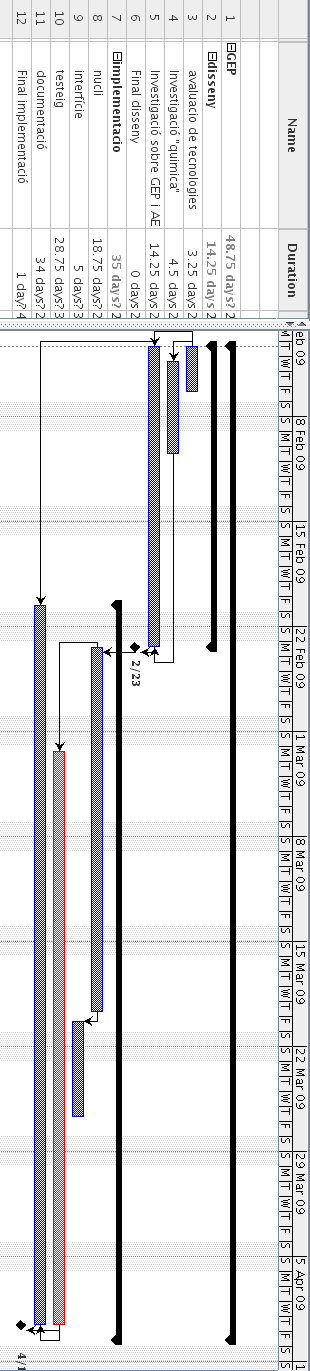
\includegraphics[scale=0.5]{gep-gantt.png}
	\end{center}
	\caption{Gantt del projecte GEP}
	\label{fig:sobreent}
\end{figure}
% section Conclusions i treball futur (end)
%\end{document}
